\chapter{Resultados y discusión}

La composición de imágenes satelitales de radiancia en la Ciudad de México (Figura~\ref{radiancetrends}) muestra cualitativamente que los niveles más altos de radiancia promedio se encuentran en la fracción norte-centro de la ciudad, lo que naturalmente, coincide con los asentamientos urbanos. Dada esta distribución, se considera que un observador está <<dentro de la ciudad>> cuando se encuentra en alguno de los Sectores Urbanos mostrados en el Mapa CL-CDMX y <<fuera de la ciudad>> cuando está fuera de ellos, lo que corresponde con suelo de conservación. 

\section{Tendencias de radiancia promedio en las alcaldías de la Ciudad de México}
\label{subsec:tendenciasradiancia}

Por efectos de representatividad se selecionaron las siguientes figuras elaboradas con el software \textit{Radiance Light Trends} que muestran las tendencias de radiancia promedio en la alcaldía Gustavo A. Madero (GAM, densamente poblada), Milpa Alta (MA, menos poblada, con mayoría de territorio en suelo de conservación) y en el polígono de CU que contiene la REPSA. El resto de las tendencias por alcaldía se encuentran en el \textbf{\autoref{chap:anexos}}.

\begin{figure}[htb]
  \centering
    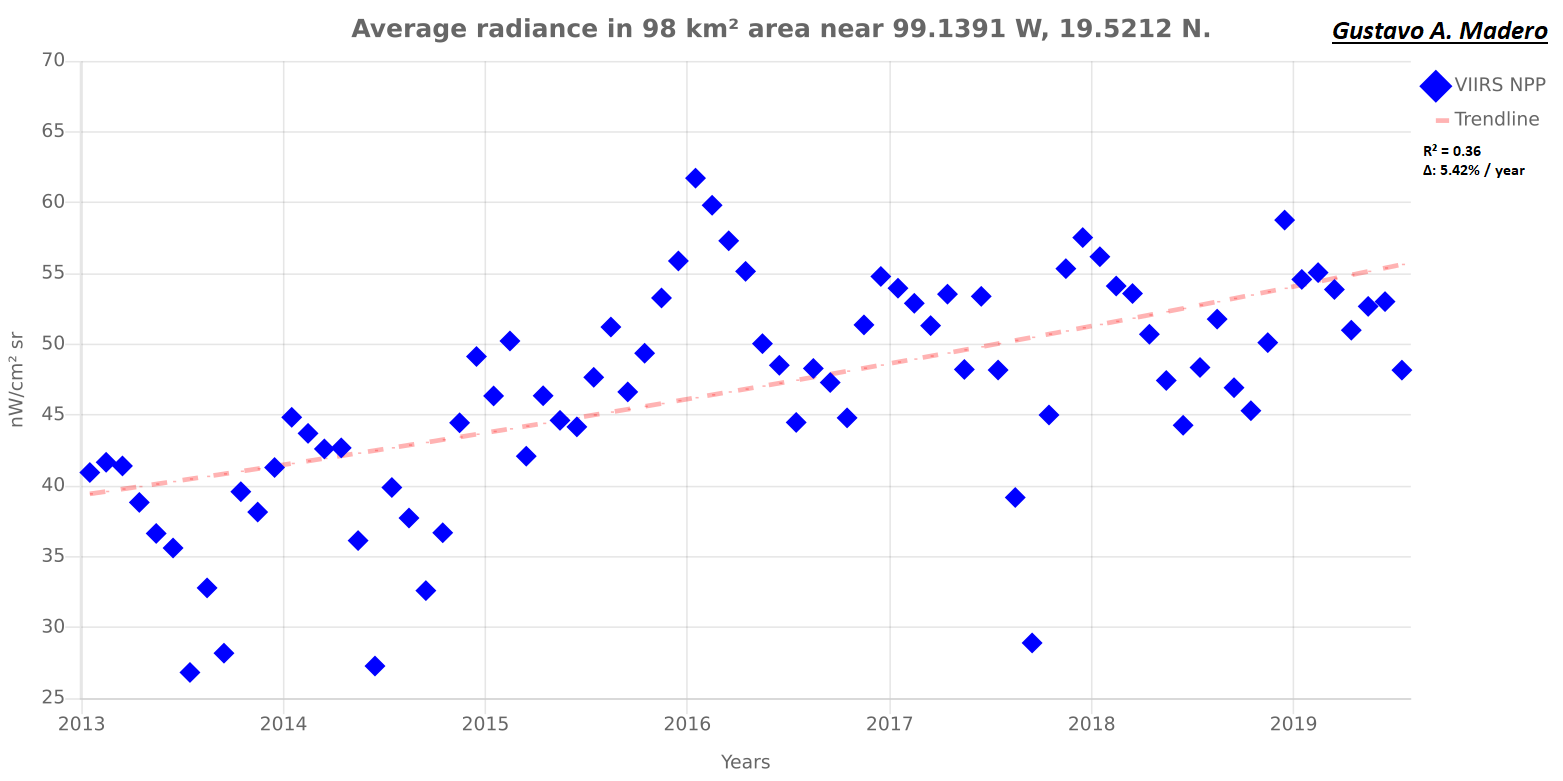
\includegraphics[width=1\textwidth]{GAM}
  \caption{Tendencia de radiancia promedio para la alcaldía GAM}
  \label{radiancetrendsgam}
\end{figure}

\newpage


\begin{figure}[H]
  \centering
    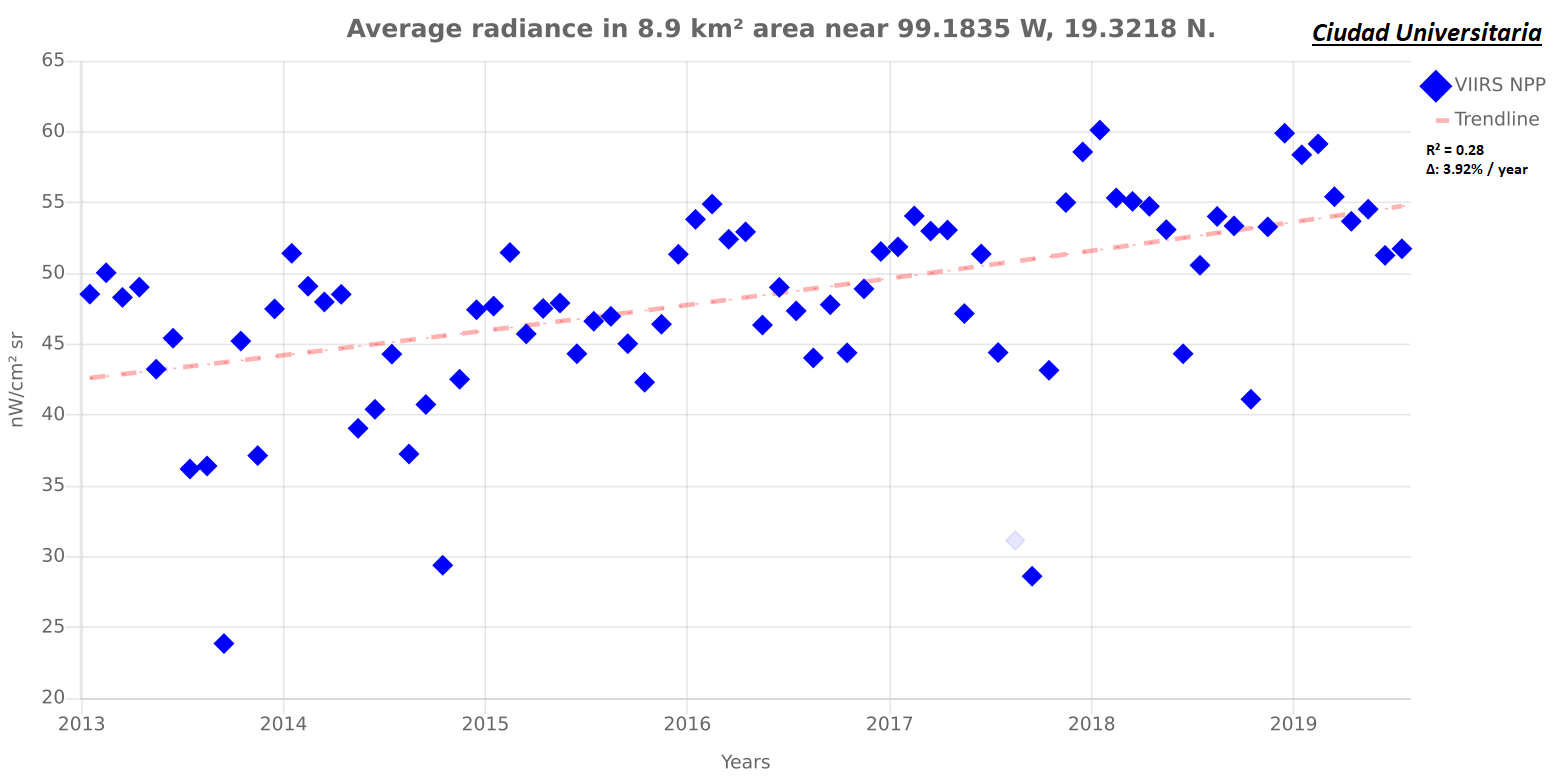
\includegraphics[width=1\textwidth]{CU}
  \caption{Tendencia de radiancia promedio para CU}
  \label{radiancetrendscu}
\vspace{20mm} 
    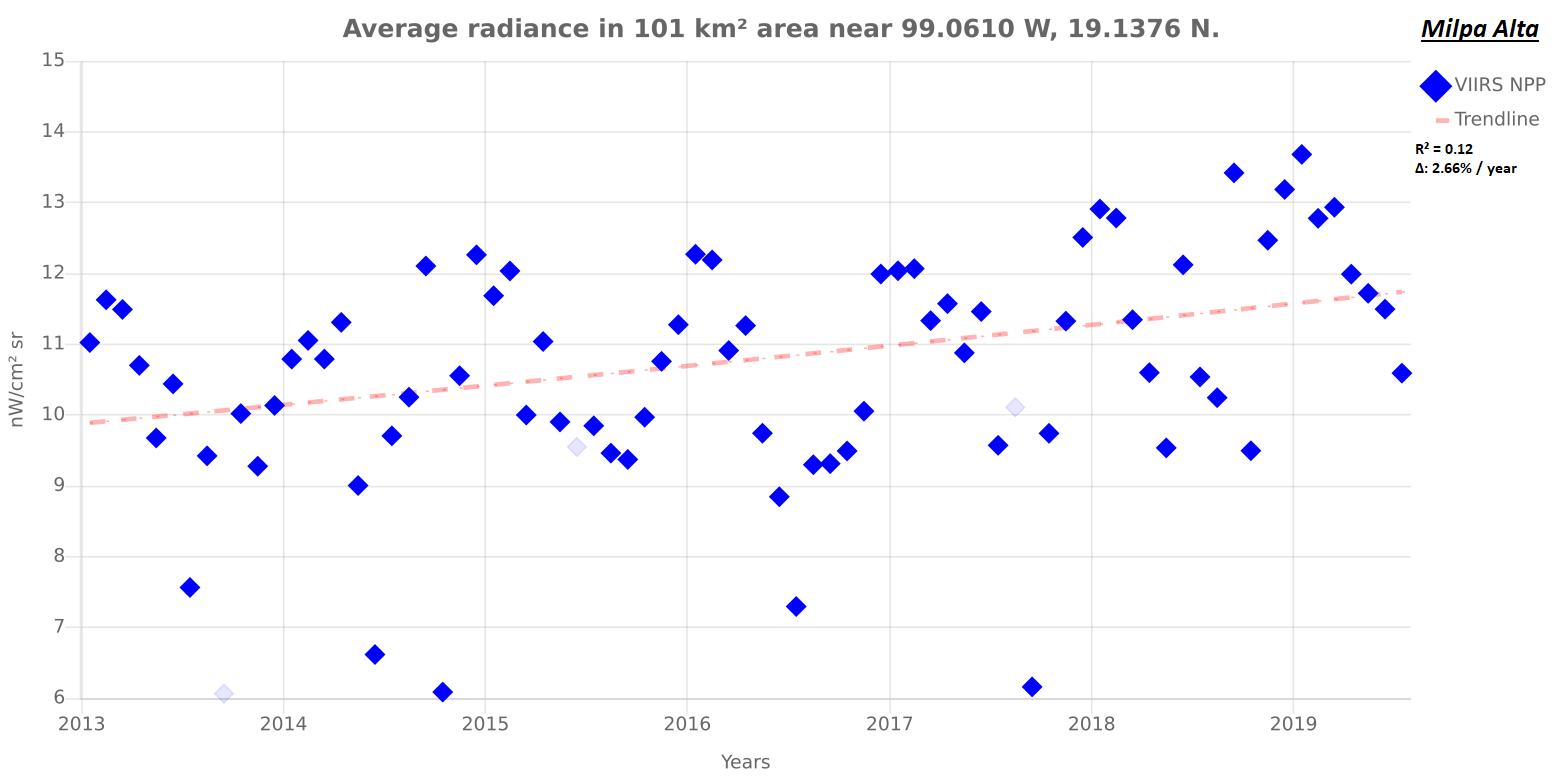
\includegraphics[width=1\textwidth]{MA}
  \caption{Tendencia de radiancia promedio para la alcaldía MA}
  \label{radiancetrendsma}
\end{figure}
\blindtext

\newpage

Como se muestra en el \textbf{Inventario de Alumbrado Público de la Ciudad de México}, hoy en día el principal tipo de fuente de luz del alumbrado público de la Ciudad de México es la lámpara de halogenuros metálicos. Sin embargo, de manera histórica, el número de luminarias y sus características han ido cambiando, lo que sumado a la fluctuación de  las luminarias residenciales y privadas ha tenido efecto en las tendencias de radiancia en las diferentes alcaldías de la ciudad.\\

De acuerdo con \cite{Universal2017} durante 2015 se destinaron 2600 millones de pesos mexicanos para el programa <<Iluminemos Tu Ciudad>>, que llevó a cabo el cambio de luminarias en vías primarias y secundarias de la Ciudad de México. Se menciona este hecho como la actualización de una <<tecnología de la década de 1990 por una más limpia>>.\\

La fuente de luz de las antiguas luminarias mencionadas era de halogenuros metálicos con un tubo de descarga de cuarzo mientras que las nuevas también tienen fuente de de halogenuros metálicos pero con la diferencia que el tubo de descarga es de cerámica, lo que algunos fabricantes mencionan 10-20\% más eficiente \citep{EMB2007}.\\

En pocas palabras, la dependencia espectral del alumbrado de la ciudad no cambió durante la aplicación del programa. En este punto es importante mencionar que la cualidad de <<limpia>> a la que los encargados del programa se refieren, no tiene nada que ver con CL sino con la diferencia en el consumo de las lámparas: mientras que las antiguas consumían 250 W, las nuevas consumen 140 W.\\ 

No obstante, durante el programa se instalaron 100 mil nuevas luminarias lo que en términos totales supone un ahorro de 27,000 kW h$^-1$ al día y 118,260 MW h$^-1$ al año; esto corresponde a menos del 1\% del consumo de energía eléctrica de la ciudad (véase la \textbf{\autoref{subsec:consumoenergiaelectrica}}). El resultado de este cálculo parece indicar que el programa no fue en realidad llevado a cabo pensando en iluminación <<más limpia>>, lo que se confirma con el conflicto de interés que lo caracterizó, en que el total de la inversión se asignó a empresas con antecedentes de incumplimiento pertenecientes a familiares del titular de Obras Públicas de la Ciudad de México de ese entonces \citep{Sinembargo2015}.\\ 

A pesar de todo, el programa <<Iluminemos Tu Ciudad>> hizo honor a su nombre y la DNB logró captarlo desde el espacio: de 2015 a 2016 se observa un marcado aumento en los niveles de radiancia promedio en la mayoría de las alcaldías (Figura~\ref{radiancetrendsgam}, \textbf{\autoref{chap:anexos}}). Mientras tanto, otras delegaciones cuya mayoría de territorio se encuentra fuera de la ciudad no muestran un crecimiento exponencial en radiancia promedio (Figura~\ref{radiancetrendsma}) debido a que en esas zonas la población es extremadamente baja. Para el caso de CU (Figura~\ref{radiancetrendscu}) se observa también un crecimiento exponencial en radiancia promedio aunque a una velocidad más lenta con respecto a la mayoría de las alcaldías.\\ 


Referente a los valores promedio de radiancia se registran los más altos en alcaldías dentro de la ciudad con el valor más extremo (86 nW sr$^{-1}$  cm$^{-2}$) obtenido para la alcaldía Venustiano Carranza en 2016, lo que no resulta extraño cuando se remite al dato destacado por el \textit{City Manager} de la Ciudad de México acerca de que, en la zona de Los Arenales en la alcaldía Venustiano Carranza <<todo está encendido>> en comparación a otras zonas de la Ciudad de México \citep{Universal2017}.\\

\newpage

Por otro lado, valores promedio de radiancia muy bajos de hasta 6 nW sr$^{-1}$  cm$^{-2}$ se registraron para la alcaldía Milpa Alta, mientras que para CU, los valores se registran alrededor de los promedios observados en otras alcaldías dentro de la ciudad.\\

Por lo tanto, los valores de radiancia promedio medidos por la DNB para la Ciudad de México están comprendidos entre 6 x 10$^{-5}$ y 8.5 x 10$^{-4}$ W sr$^{-1}$ m$^{-2}$, valores por encima del máximo natural registrado (10$^{-6}$ W sr$^{-1}$  m$^{-2}$), por lo que se puede hablar de la presencia de CL en todo el territorio de la Ciudad de México.\\ 

El futuro en cuestiones de CL no pinta bien al pensar en el panorama planteado por la Agencia de Gestión Urbana que sumándose a la tendencia global de las ciudades, pretende instalar <<dispositivos que iluminan mejor y son más eficientes como la tecnología LED>> en vías primarias de la ciudad \citep{Universal2017}. Véase la \textbf{\autoref{subsec:consecuenciascl}} en que se reporta el LED como la fuente de luz con mayor potencial en términos de CL.\\ 


\section{Gráficas tipo \textit{all sky} de distribución de radiancia}

En esta sección se enfoca el problema de la CL desde otra perspectiva diferente a las mediciones promedio satelitales, se lleva a cabo el análisis del brillo del cielo nocturno percibido por un observador en superficie de acuerdo con las salidas del modelo \textit{SkyGlow}.\\ 

Para tales análisis se seleccionaron los mismos casos particulares de la sección anterior: un observador dentro de la alcaldía Gustavo A. Madero (coordenadas: 19.47\grad, -99.14\grad), alcaldía Milpa Alta (coordenadas: 19.09\grad, -99.15\grad) y la Zona Núcleo Oriente de la REPSA dentro de CU(coordenadas: 19.31\grad, -99.18\grad).\\

En la Figura~\ref{1} se muestran los resultados de la distribución angular para condiciones de cielo despejado para dos escenarios: con FP y con EC. Para todos los casos se observan altos valores de radiancia en el horizonte prácticamente a lo largo de todo el ángulo acimutal.\\

Nótese el caso de MA en que los valores de radiancia son menores a los casos de GAM y CU, lo cual es debido a que la distancia del observador en MA a las zonas más brillantes de la ciudad es mayor con respecto a los otros casos y que, además, el flujo de luz en MA hacia la atmósfera es menor.\\

El efecto de las EC es claro para los casos de GAM y CU en los que se observa que son responsables del aumento del brillo en el cenit, lo que se atribuye al valor bajo de ASY, lo que facilita la dispersión isotrópica.\\

Recuérdese que los valores de todas las gráficas tipo \textit{all sky} están reportados en escala logarítmica. En el caso de las figuras analizadas en esta sección se tienen valores de radiancia entre 1.36 x 10$^{-3}$ W sr$^{-1}$ m$^{-2}$ (en MA) y 1.83 x 10$^{-2}$ W sr$^{-1}$ m$^{-2}$ (en GAM).\\

\newpage

\begin{figure}[H]
  \centering
    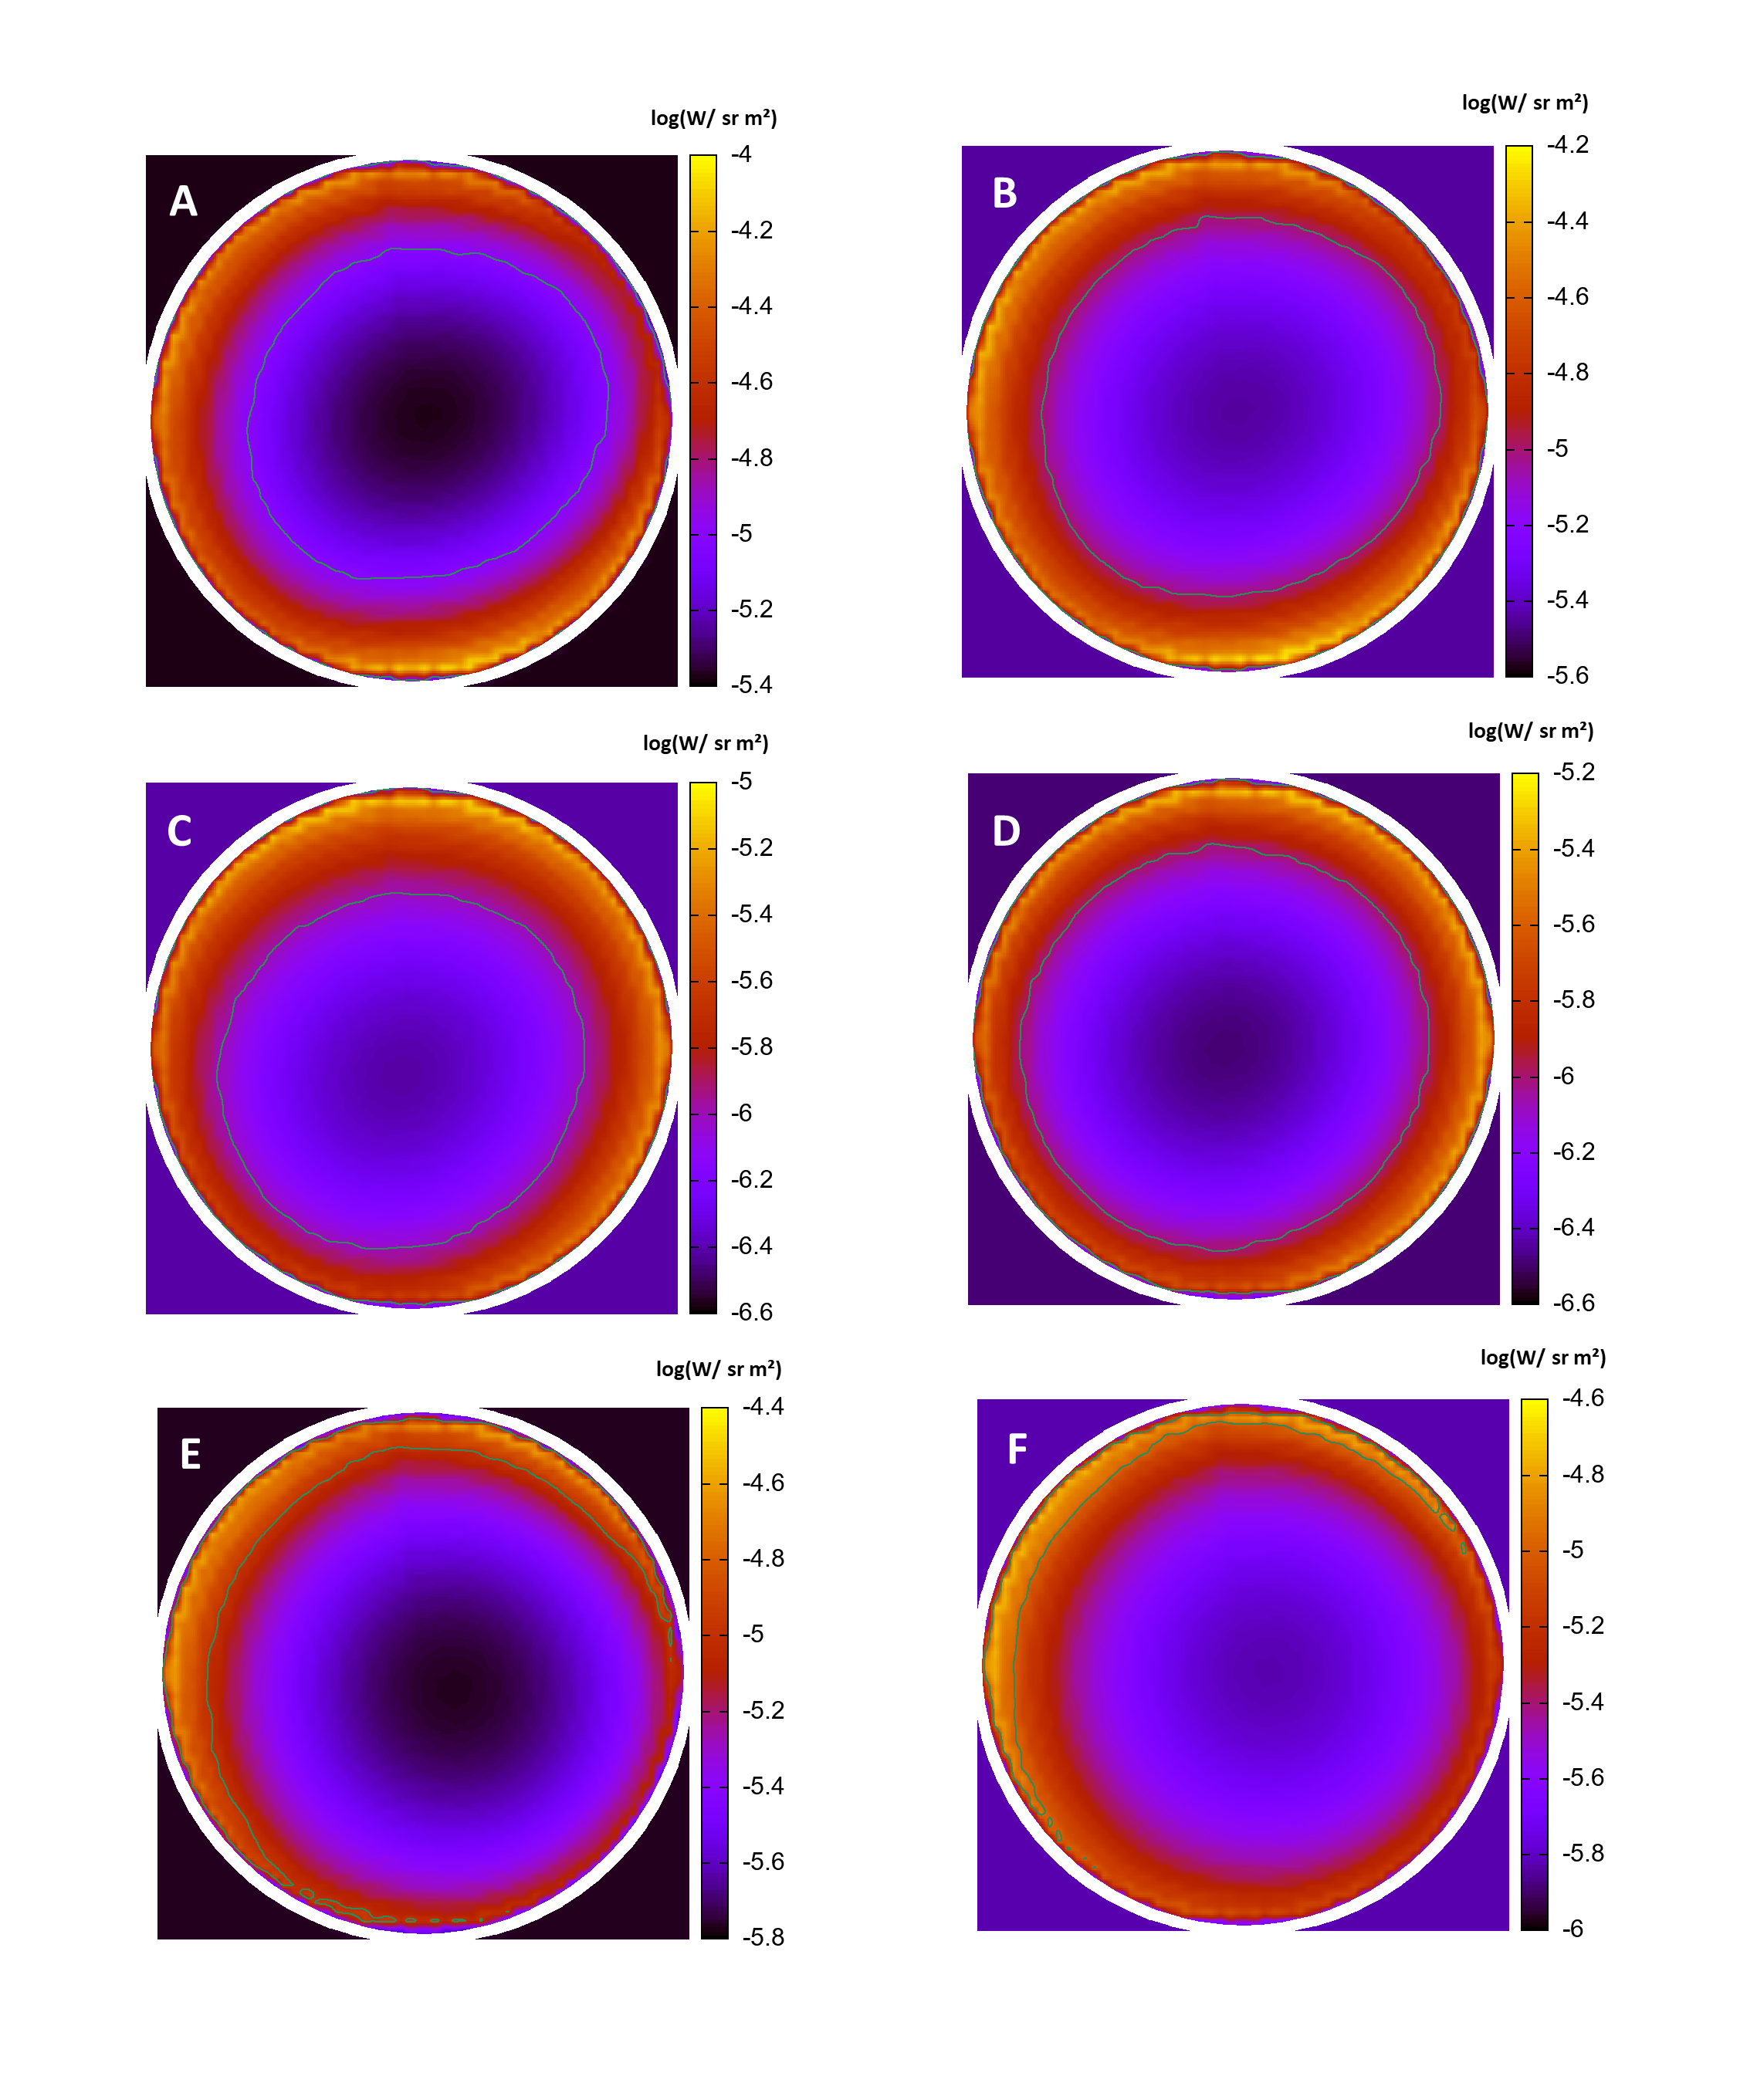
\includegraphics[width=1\textwidth]{1}
  \caption{Gráficas tipo \textit{all sky} para condiciones de cielo despejado con A) FP para GAM, B) EC para GAM, C) Caso de A) para MA, D) Caso de B) para MA, E) Caso de A) para CU y F) Caso de B) para CU} 
  \label{1}
\end{figure}


\newpage

\section{Experimentos numéricos}

Con el fin de inferir la influencia del aerosol atmosférico y la nubosidad en el brillo del cielo nocturno, se construyeron diferentes escenarios tomando como referencia los mismos observadores en superficies de la sección anterior.\\

Con respecto a la influencia del aerosol atmosférico se tomaron las condiciones observadas en la climatología para la Ciudad de México (véase la \textbf{\autoref{subsubsec:propiedadesopticasaerosol}}). Para todos los casos se observa una reducción preferencial en la radiancia del horizonte en determinados ángulos acimutales con respecto a condiciones de FP. Sin embargo, en otros ángulos acimutales se tiene un aumento drástico en la radiancia en el horizonte (valores entre 2.09 x 10$^{-3}$ W sr$^{-1}$ m$^{-2}$ (en MA) y 2.72 x 10$^{-2}$ W sr$^{-1}$ m$^{-2}$ (en GAM y CU)).\\

En particular, para GAM se observa un reducción gradual en la radiancia en el cenit conforme pasan las estaciones de Invierno Seco, Primavera Seca y Temporada Lluviosa (Figura~\ref{2}), para MA se observa la misma reducción pero comenzando desde Temporada Lluviosa (Figura~\ref{3}) y, para CU comenzando desde Primavera Seca (Figura~\ref{4}). Esta diferencia en comportamiento se puede explicar remitiéndose a las funciones $\Gamma$ y $T$ del modelo que caracterizan la distribución angular de la radiancia y su atenuación atmosférica con base a la posición del observador, el AOD y $\alpha$ (parámetros que cambian significativamente en cada escenario).\\

Con respecto a la influencia de la nubosidad se observa en todos los casos una reconfiguración total de la distribución angular de la radiancia. Conforme la nube es más baja con respecto al observador los valores de randiancia aumentan drásticamente con respecto a las condiciones de FP.\\

En particular para GAM los valores extremos de radiancia aumentan de 1.83 x 10$^{-2}$ W sr$^{-1}$ m$^{-2}$ hasta 2.72 x 10$^{-2}$ W sr$^{-1}$ m$^{-2}$ (Figura~\ref{5}). Para MA de 6.73 x 10$^{-3}$ W sr$^{-1}$ m$^{-2}$ a 1.49 x 10$^{-2}$ W sr$^{-1}$ m$^{-2}$ (Figura~\ref{6}) y para CU de 1.22 x 10$^{-2}$ W sr$^{-1}$ m$^{-2}$ a 2.47 x 10$^{-2}$ W sr$^{-1}$ m$^{-2}$ (Figura~\ref{7}). Resultan interesantes los casos de MA y CU en que la nubosidad crea un efecto de enmascaramiento de radiancia en regiones del horizonte de donde proviene menos luz.\\

Como se aborda en \textbf{\autoref{subsec:tendenciasradiancia}} por el potencial ahorro económico que supone, mundialmente se está llevando a cabo una sustitución de instalaciones de alumbrado público cambiando fuentes tradicionales a LED. Entre otros motivos que tienen que ver con la susceptibilidad de un gran número de organismos a las longitudes de onda corta, los LEDs son la fuente de luz con mayor potencial en términos de CL ya que las longitudes de onda corta que emite se transportan más eficientemente en la atmósfera por acción de la dispersión de Rayleigh.\\

En la Figura~\ref{8} se observa que al simular el cambio de iluminación de la ciudad a LED, en todos los casos ocurre un marcado aumento en los valores de radiancia con respecto a las condiciones de FP.\\

\newpage

\subsection{Influencia del aerosol atmosférico en la distribución de radiancia}

\begin{figure}[H]
  \centering
    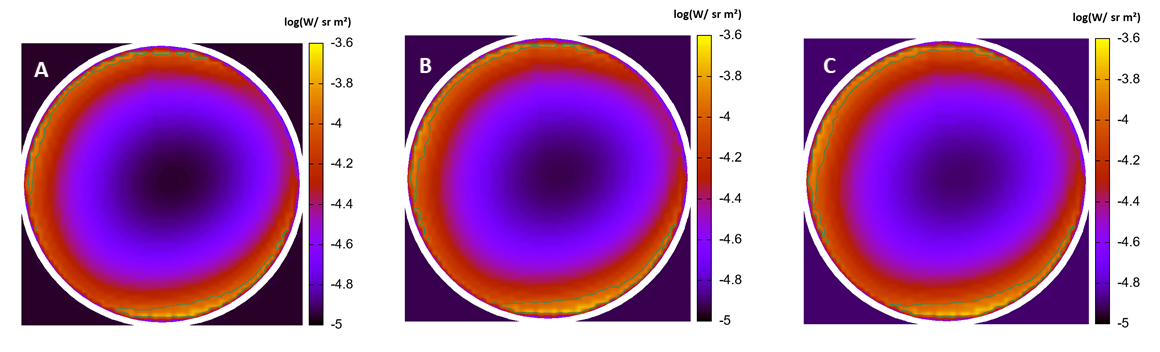
\includegraphics[width=1\textwidth]{2}
  \caption{Gráficas tipo \textit{all sky} para condiciones de cielo despejado para GAM en A) Invierno Seco, B) Primavera Seca y C) Temporada Lluviosa} 
  \label{2}
\end{figure}}

\begin{figure}[H]
  \centering
    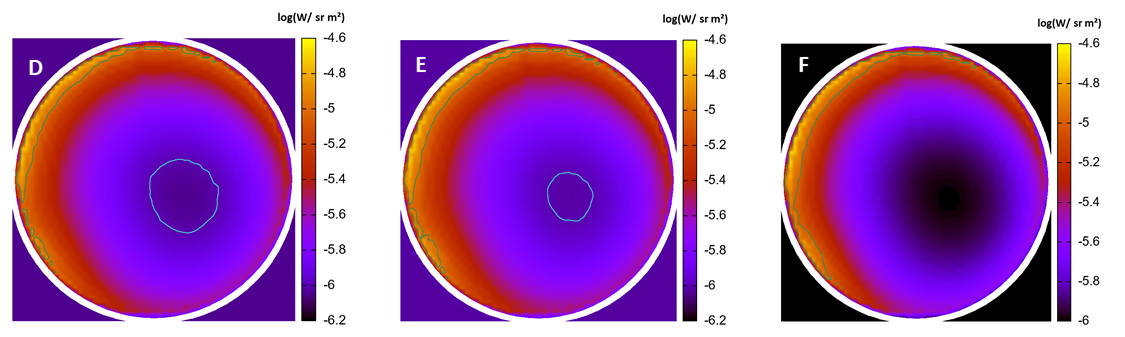
\includegraphics[width=1\textwidth]{3}
  \caption{Gráficas tipo \textit{all sky} para condiciones de cielo despejado para MA en A) Invierno Seco, B) Primavera Seca y C) Temporada Lluviosa} 
  \label{3}
\end{figure}

\begin{figure}[H]
  \centering
    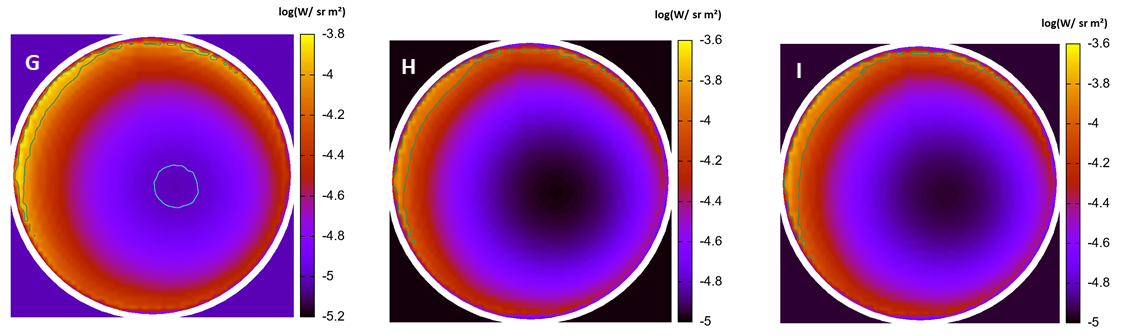
\includegraphics[width=1\textwidth]{4}
  \caption{Gráficas tipo \textit{all sky} para condiciones de cielo despejado para CU en A) Invierno Seco, B) Primavera Seca y C) Temporada Lluviosa} 
  \label{4}
\end{figure}

\newpage

\subsection{Influencia de la nubosidad en la distribución de radiancia}

\begin{figure}[H]
  \centering
    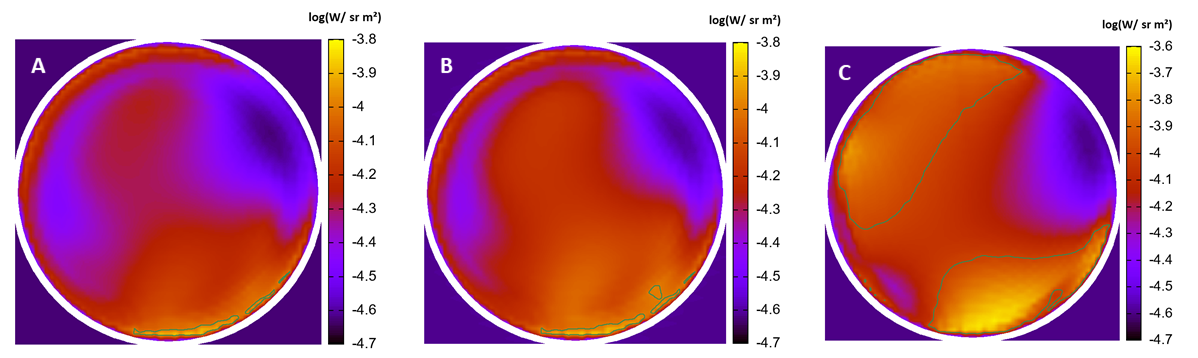
\includegraphics[width=1\textwidth]{5}
  \caption{Gráficas tipo \textit{all sky} para condiciones de cielo nublado para GAM con A) \textit{altocumulus}, B) \textit{altostratus} y C) \textit{stratus}} 
  \label{5}
\end{figure}

\begin{figure}[H]
  \centering
    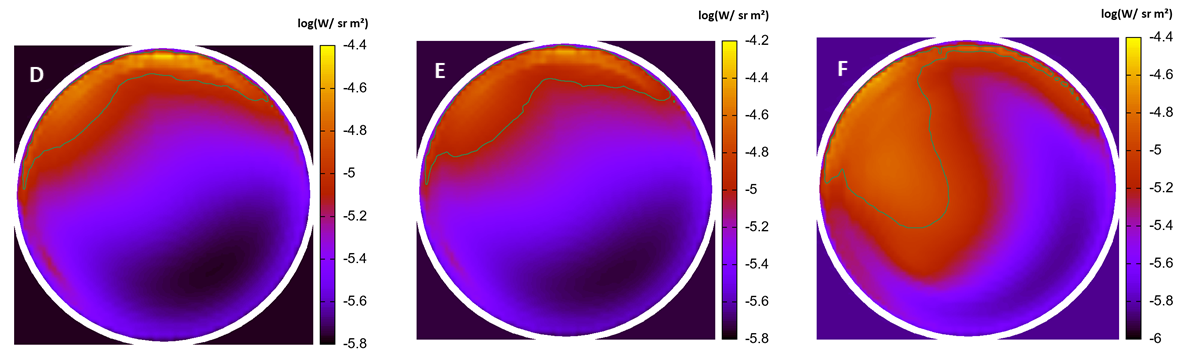
\includegraphics[width=1\textwidth]{6}
  \caption{Gráficas tipo \textit{all sky} para condiciones de cielo nublado para MA con A) \textit{altocumulus}, B)  \textit{altostratus} y C) \textit{stratus}} 
  \label{6}
\end{figure}

\begin{figure}[H]
  \centering
    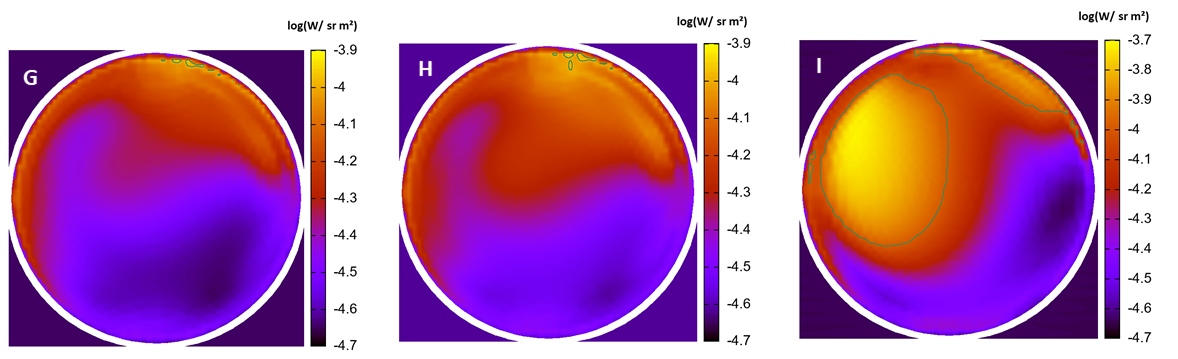
\includegraphics[width=1\textwidth]{7}
  \caption{Gráficas tipo \textit{all sky} para condiciones de cielo nublado para CU con A) \textit{altocumulus}, B) \textit{altostratus} y C) \textit{stratus}} 
  \label{7}
\end{figure}

\newpage

\subsection{Cambio del tipo de luminarias en la Ciudad de México}

\begin{figure}[H]
  \centering
    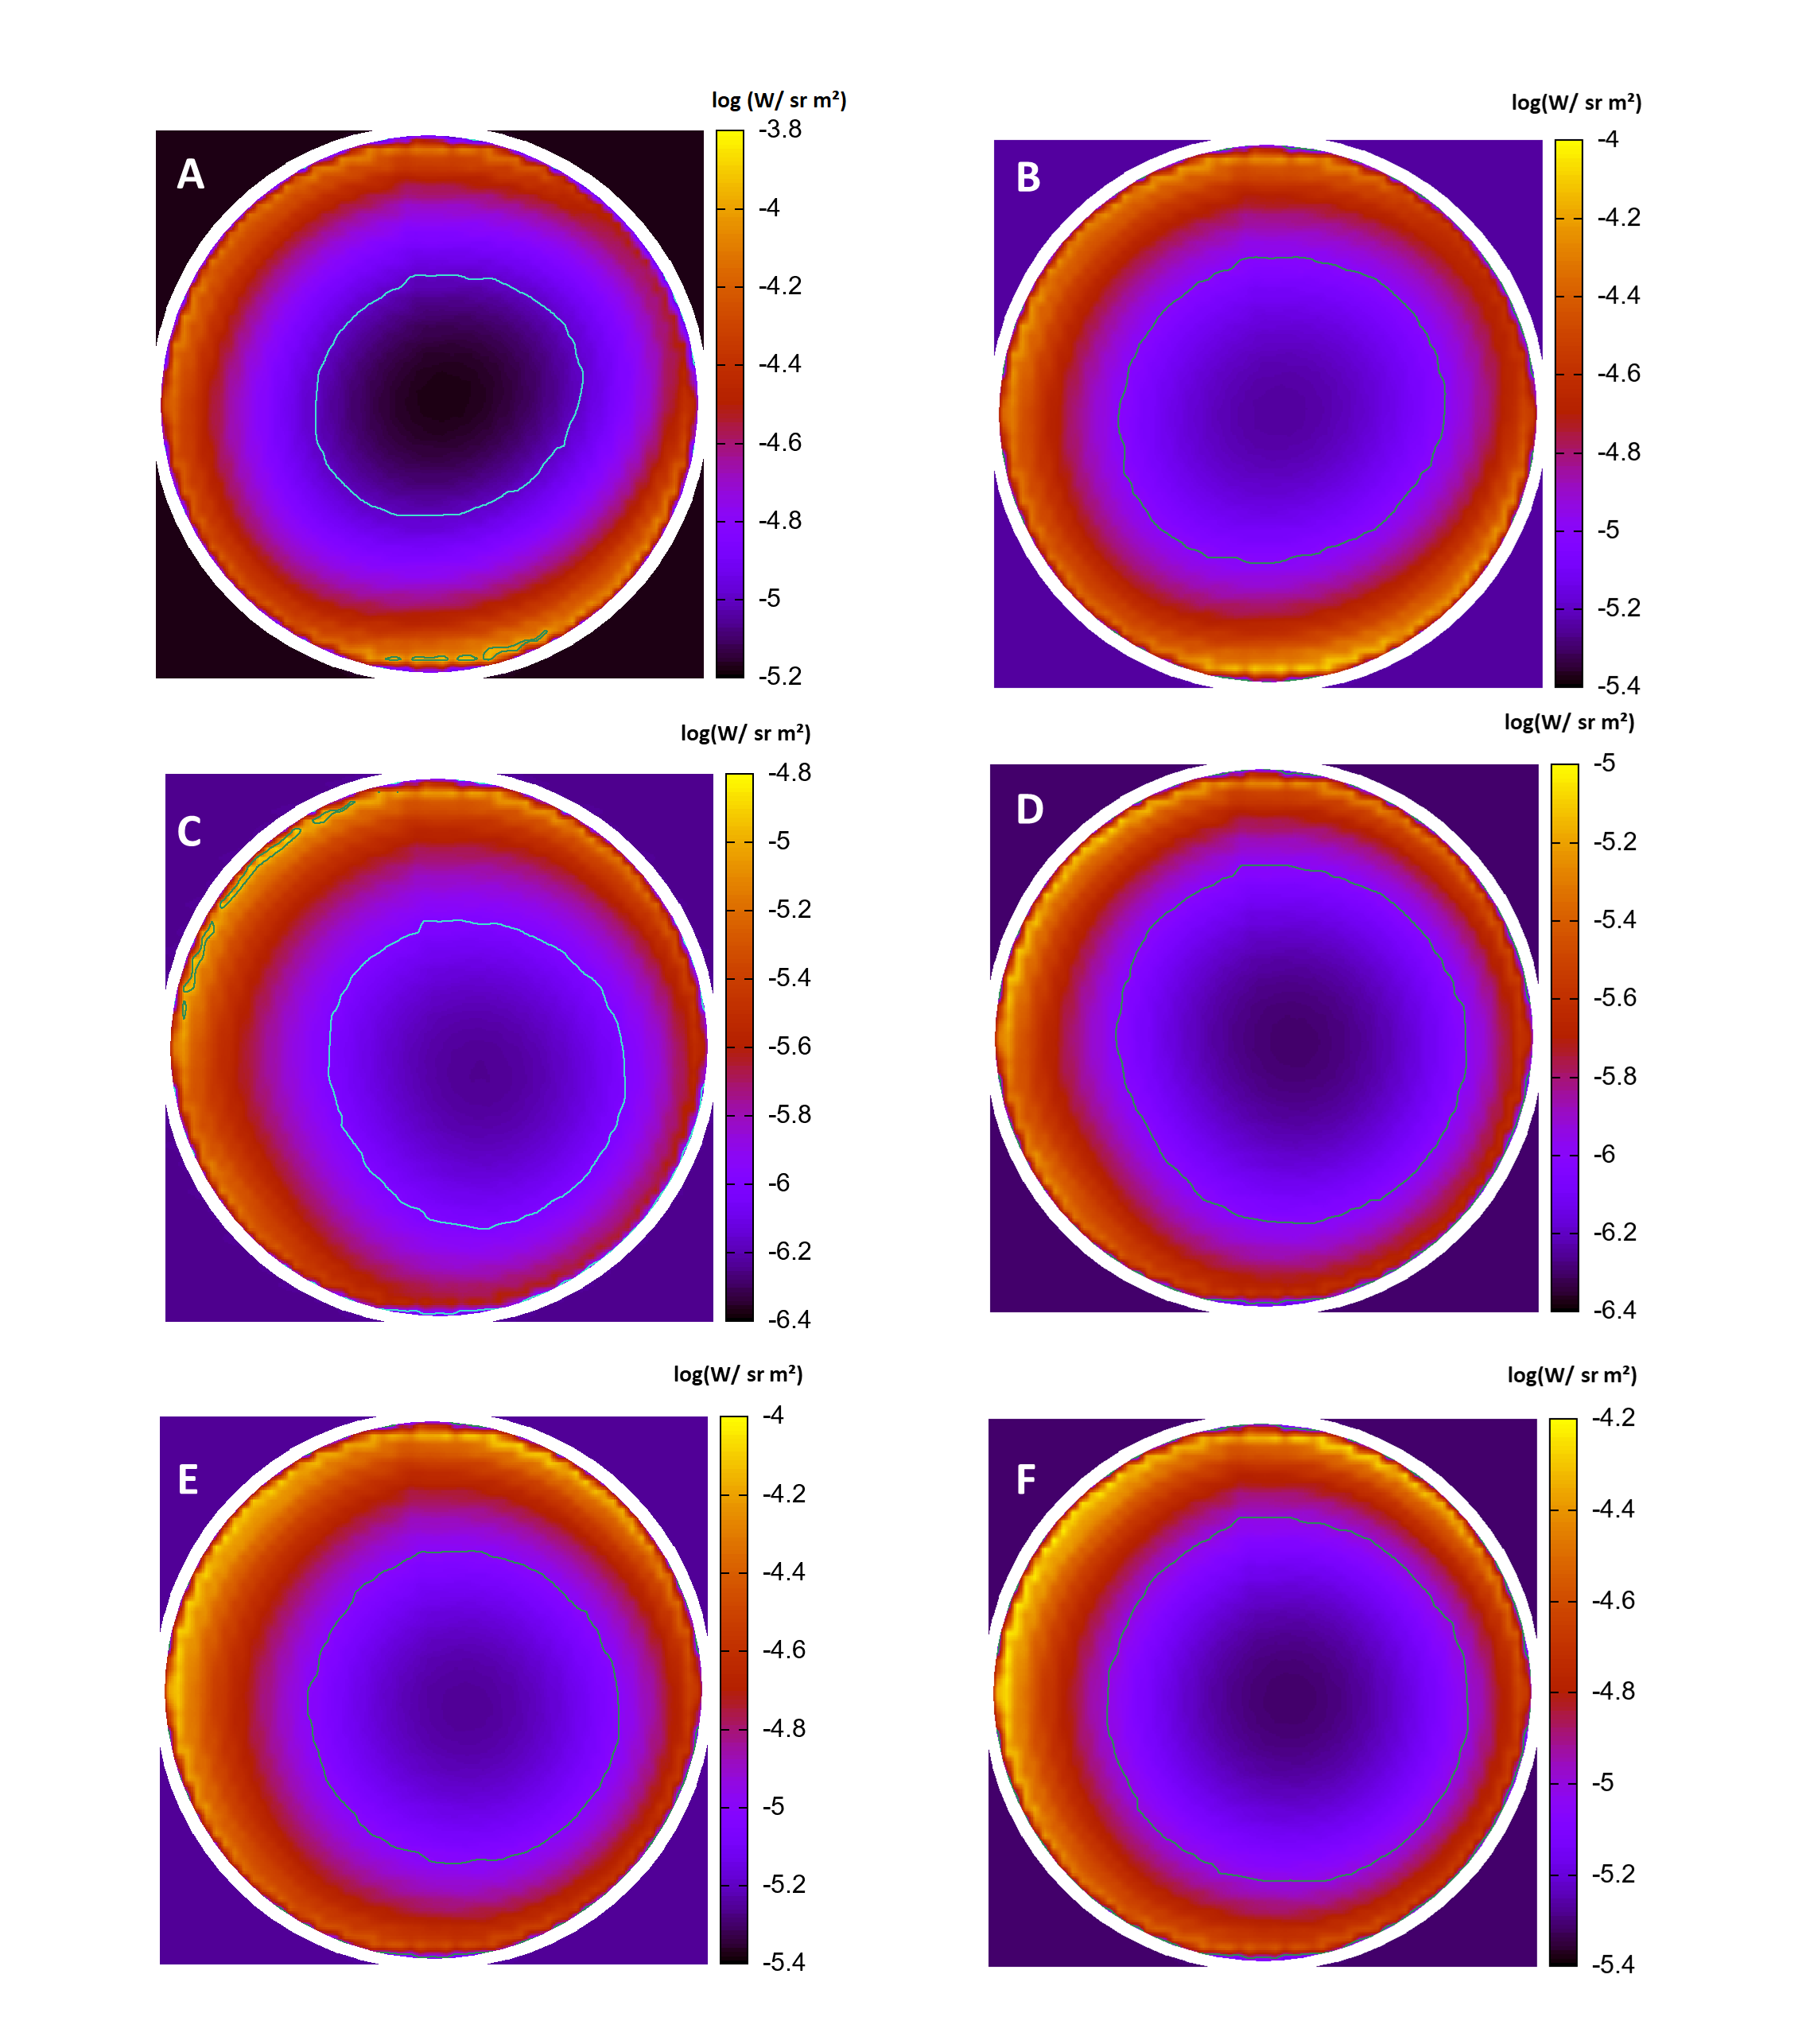
\includegraphics[width=1\textwidth]{8}
  \caption{Gráficas tipo \textit{all sky} para condiciones de cielo despejado con tipo de luminaria LED con A) FP para GAM, B) EC para GAM, C) Caso de A) para MA, D) Caso de B) para MA, E) Caso de A) para CU y F) Caso de B) para CU} 
  \label{8}
\end{figure}

\newpage

\section{Mapa CL-CDMX}
\label{sec:mapacl}

Para efectos de evaluación teórica de los efectos de la distribución de radiancia en el cielo nocturno (brillo del cielo) sobre la irradiancia difusa percibida por un observador en superficie se construyó el \textbf{Mapa Teórico de Contaminación Lumínica de la Ciudad de México} con las salidas del modelo \textit{SkyGlow} (Figura~\ref{8}).\\

Advertencia: los valores de irradiancia presentados en el mapa no son un indicativo directo de los niveles de CL, más bien, son representativos de la tendencia de CL en el rango visible del EE. De manera tradicional los efectos directos de la CL sobre la biodiversidad se efectúan empleando mediciones fotométricas que quedan restringidas en el ámbito de la visión humana y, por lo tanto, se pierde mucha información en el proceso; un aspecto novedoso que ofrece la base teórica del Mapa CL-CDMX es la posibilidad de mapear valores de irradiancia en superficie aplicando filtros específicos basados en la visión de diferentes especies, es decir: generar mapas de cómo perciben el brillo del cielo nocturno diferentes especies en diferentes lugares de la ciudad.\\

Lo anterior es posible efectuarlo de acuerdo con \cite{Solano2013} a través de la modificación de la ecuación \ref{eq:2.5} obteniendo:

\begin{equation}
D_{\lambda} = \int_{\lambda_{1}}^{\lambda_{1}} \zeta(\lambda) \int_{z = 0}^{z =\pi/2} \int_{\phi = 0}^{\phi = 2\pi} I_{\lambda} (z, \phi) \: sen \,z \: dz \: d\phi
\end{equation}\\


En donde $\zeta(\lambda)$ es la respuesta espectral de una especie en particular siendo una función de su tipo de visión (fotópica, mesópica o escotópica).\\

Por otro lado, el Mapa CL-CDMX permite evaluar la correcta reproducción de las tendencias observadas de CL por la DNB (Figura~\ref{radiancetrends}). En general, se observa una reproducción muy fiel al tener los niveles más bajos de irradiancia fuera de la ciudad y los mayores en el Centro de la ciudad integrado por los Sectores Centro, Roma, Tlatelolco, Buenavista y Morelos. Nótese que las regiones en color blanco corresponden a zonas no iluminadas, como el sur de la Ciudad de México y ANPs dentro de la ciudad, o con iluminación especial (no correspondiente al alumbrado público) como el Aeropuerto Internacional de la Ciudad de México, CU, Reclusorio Norte y el Colegio Militar.\\

Por último, se propone el Mapa CL-CDMX como un antecedente para la zonificación que necesita cualquier legislación en materia de CL para la Ciudad de México (véase la \textbf{\autoref{subsec:marcoregulatorio}}). Sumado a todo, se hace un llamado a abordar el problema de la CL y su mitigación a través de la zonificación basada en el enfoque socioecosistémico abordado en la \textbf{\autoref{subsec:enfoquesocioecosistemico}}: no porque una zona sea altamente comercial o turística significa que sus fuentes de luz puedan ser de cualquier tipo, tiene que pensarse en que la especie humana coexiste con otras miles de especies en un mismo espacio y que nuestros caminos y calles son los suyos también, la sustentabilidad no se construye para el futuro sino para hoy, las ciudades no son estructuras inmutables que tengan que reproducir esquemas antropocentristas sino procesos de la naturaleza. 

\newpage

\vspace{100mm} 

\begin{figure}[H]
  \centering
    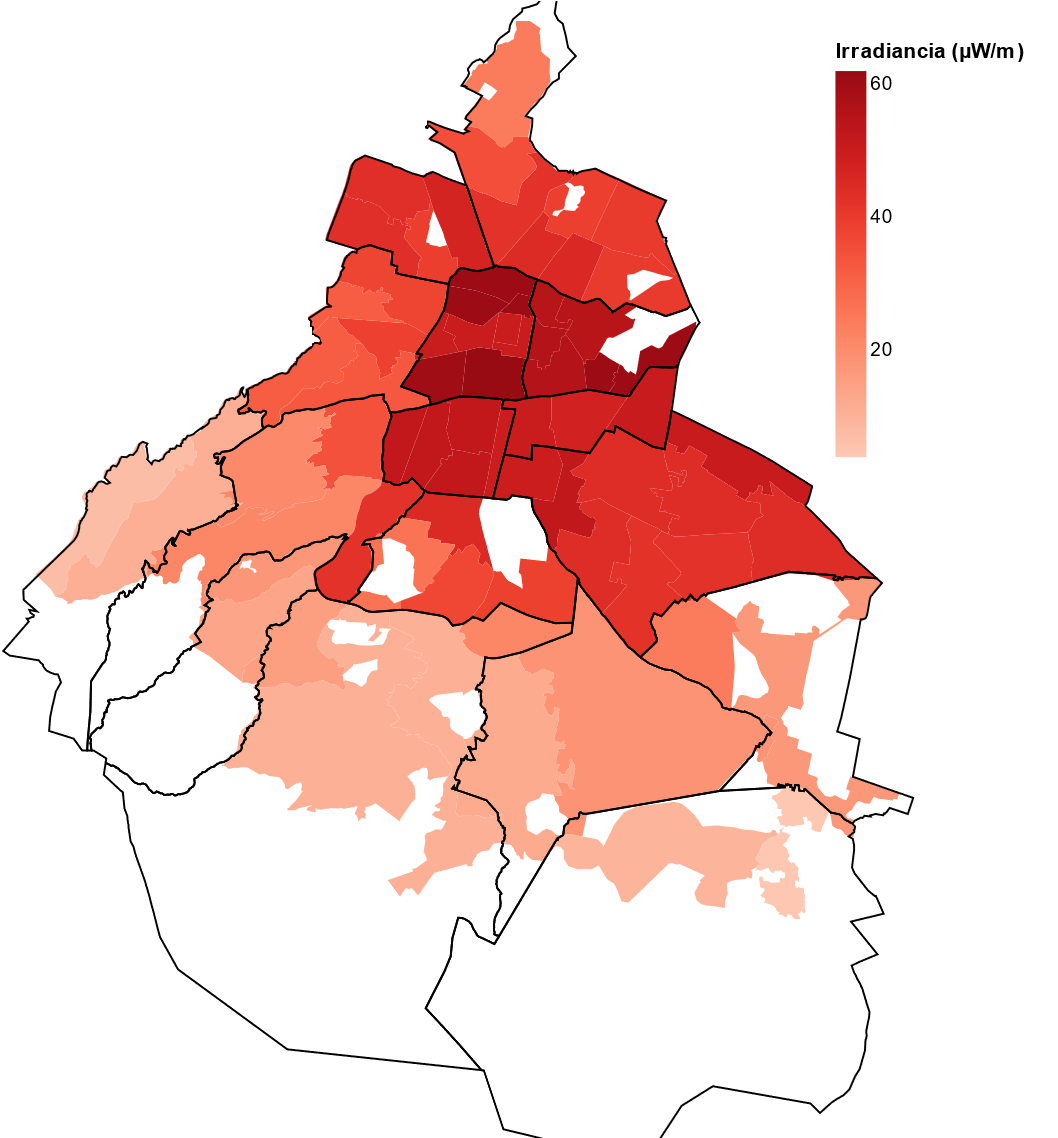
\includegraphics[width=1\textwidth]{MapaCLCDMX}
  \caption{Mapa CL-CDMX} 
  \label{MapaCLDMX}
\end{figure}

\newpage